\documentclass[12pt]{article}
%\documentclass[8pt,twocolumn]{article}

\usepackage{graphicx}
\usepackage{comment}
\usepackage{float}
\usepackage{hyperref}
\usepackage[authoryear]{natbib}
\usepackage{setspace}
\usepackage{mathtools}
%\usepackage{aas_macros}
\usepackage{amssymb}
\usepackage{textcomp}
\usepackage{siunitx}

\title{Acousto-Optical Tunable Filter Atmospheric Imager for Determination of Aerosol Extinction}

\author{Brenden J Elash, Adam E Bourassa, Douglas A Degenstein}

\begin{document}
\renewcommand\bibname{BiBTex.bib}

\maketitle

\section{Introduction}

The Atmospheric Limb Imager (ALI) is a prototype atmospheric instrument developed at the University of Saskatchewan with the long term goal for a satellite instrument in the future with the purpose to gather high resolution horizontal and vertical aerosol microphysics profiles, including extinction and particle size. The purpose of the ALI prototype is to test and verify the use of an Acousto-Optical Tunable Filter (AOTF), the fundamental technology behind ALI, in a space environment and to gather atmospheric sulfate aerosol profiles with high spacial resolution. ALI will measure light from the atmosphere through the limb geometry which measures the radiance from scattered sunlight from the sunlit atmosphere. ALI is a single channel instrument measuring radiance from the visible to the near infrared wavelengths (650-950~nm) and through successive images build spectral information. The system uses a telescoptic front end to pass collimated light through the AOTF which is then focused onto the the detector. The AOTF has the unique property of separating the incoming radiance into each of its linear polarized components and rotating the the selected wavelength polarization by 90\si{\degree} allowing one to recover some polarization information of the incoming radiance. The ALI prototype was completed in August of 2014 and a stratospheric balloon test flight from the Canadian Space Agency (CSA) balloon launch facility in Timmins Ontario onboard the CNES gondola platform occurred on September 20, 2014.

The atmosphere has been monitored in several different geometries throughout the history. Occultation was one of the first methods used on satellite instrumentation to measure atmospheric species including ozone notable instruments included SAM II \citep{McCormick1979}, SAGE II \citep{McCormick1987}, and SAGE III \citep{Thomason2003}. Different instrumentation techniques were also put into space to acquire atmospheric data for different species with differing resolutions and quantity of data that could be acquired in a single day. One such geometry is the limb scatter geometry which measures radiance from the sunlite atmosphere as it scatters and interacts with molecules. However, the limb scatter geometry has a complexity that requires a foreword model to be able to accurately compute the scattering interactions, both single and multiple, between different constituents in order to be able to acquire any useful atmospheric information form the recorded data. Two instruments from the previous generation of remote sensing instruments have successfully used limb scatter to determine atmospheric parameters, the Optical Spectrograph and InfraRed Imaging System (OSIRIS) an Canadian instrument onboard the Odin satellite \citep{Llewellyn2004} and SCanning Imaging Absorption spectroMeter for Atmospheric CHartographY (SCIAMACHY) onboard the ENVISAT \citep{Bovensmann1999} which are grating spectrometers that can only acquire data at a single altitude at a time so a series of exposures is required to create a vertical profile. The new proposed method with ALI allows for a two dimensional spacial images of a single wavelength polarized light to be acquired giving both vertical and horizontal resolution of the environment through the use of the innovative AOTF technology.

Sulfuric aerosol is a fundamental portion of the global climate balance, work by \cite{Andreae2005} has show that global warming has not been as drastic as perviously expected due to the high amounts of aerosol in the stratosphere currently due to the high volcanic activity. Aerosol is a spherical partial that scattered incoming radiance away from the surface of the planet causing an overall cooling effect which is dependant on particle size distribution \citep{Kiehl1993}. This effect is fully defined by aerosol microphysics requiring accurate knowledge of concentration and particle size distributions. Furthermore, high resolution aerosol measurements are required in order to be able to determine aerosol extinction ratio during high aerosol loading due to the long path length and high amount of attenuation due to aerosol scattering. The method of aerosol transportation across the tropopause are not completely understood, recently after the 2011 eruption of Nabro it was determined that the asian monsoon has the ability to penetrate through the thermal boundary and ejected aerosol from the Nabro plume into the stratosphere \citep{Bourassa2012c}. Current generation instrumentation does not have the necessary resolution needed for current scientific needs and additional horizontal and vertical resolution will allow the determination of aerosol loading from volcanic and anthropogenic sources casuing a cooling effect  and account for losses from the stratosphere due to transportation that will result in an overall heating of the planet's surface. ALI, a prototype for a next generation of instruments will address the much needed horizontal and vertical resolution improvement required to help answer questions about global climate.

In this paper the first section will outline the technology behind the AOTF used within the ALI system and then describe the optical design behind ALI and an ulterior optical presentation including the comparison with the Belgium instrument ALTIUS. Followed by ALI's maiden flight onboard the CNES CARMEN gondola from the CSA balloon launch facility in Timmins, Ontario including the conditions and trajectory of the flight day, and the measurement taken during the campaign including an analysis of the conversion from raw measurement into calibrated data. Lastly, an retrieval algorithm for aerosol extinction and particle size parameters will be outlined and then preformed on the from the data for the campaign.

\section{Instrument Design}

\subsection{Acouto-Optical Tunable Filter}



%where $\mathbf{k}_{i}$ and $\mathbf{k}_{d}$ are the wave vectors for the incoming and diffracted light and $\boldsymbol\kappa$ is the acoustic wave vector. These wave vectors can be described by
%\begin{equation}
%    \ k_{i} = \frac{2\pi n_{i}}{\lambda}
%    \label{eqn:3.1:incomingWavevector}
%\end{equation}
%\begin{equation}
%    \ k_{d} = \frac{2\pi n_{d}}{\lambda}
%    \label{eqn:3.1:diffractedWavevector}
%\end{equation}
%\begin{equation}
%    \ \kappa = \frac{2\pi F}{\nu}
%    \label{eqn:3.1:acousticWavevector}
%\end{equation}
%where $n_{i}$ and $n_{d}$ are the indices of refraction of incoming and diffracted light. Finally $\lambda$ is the wavelength of light in a vacuum. It will be assumed that the extraordinary light is undergoes the momentum matching through the device. This causes the above refractive indices defined above to be
%\begin{equation}
%    \ n_{i} = \left( \frac{\sin^{2}(\theta_{i}+\alpha)}{n_{e}^{2}} + \frac{\cos^{2}(\theta_{i}+\alpha)}{n_{o}^{2}} \right)^{-\frac{1}{2}}
%    \label{eqn:3.1:incomingIndexOfRefraction}
%\end{equation}
%\begin{equation}
%    \ n_{d} = n_{o}
%    \label{eqn:3.1:diffractedIndexOfRefraction}
%\end{equation}
%where $n_{e}$ and $n_{o}$ are the indices of refraction for the extraordinary and ordinary polarizations of the incoming light and $\alpha$ is the cut angle relative to the piezoelectric transducer and the optical axis. For a crystal, like TeO$_{2}$, the difference in the index of refraction is small and can be approximated as \citep{Voloshinov2007}
% \begin{equation}
%    \ n_{i} = n_{o} + \Delta n\sin^{2}(\theta_{i}+\alpha)
%    \label{eqn:3.1:incomingIndexOfRefractionApprox}
%\end{equation}
%where $\Delta n$ is the difference between the extraordinary and ordinary indices of refraction (ie $\Delta n = n_{e} - n_{o}$). The wave vectors, seen in \autoref{fig:3.1:ATOFWavevectors}, of the system need to follow the momentum matching criteria from \autoref{eqn:3.1:phaseMatching}. Separating the wave vectors into their directional components with respect to the cut angle, $\alpha$, the tangential and perpendicular directions respectively are
%\begin{equation}
%    \ k_{i}\cos\theta_{i} = {k}_{d}\cos\theta_{d}
%    \label{eqn:3.1:wavevectorsTangentalDirection}
%\end{equation}
%\begin{equation}
%    \ k_{i}\sin\theta_{i} + \kappa = {k}_{d}\sin\theta_{d}
%    \label{eqn:3.1:wavevectorsPerepndicularDirection}
%\end{equation}

The use of an AOTF for an image system has several distinct advantages due to its low mass, fast stabilization times of a few microseconds, and no moving parts and has only recently become possible thanks to improvements to non-collinear acosto devices with the use of birefringent materials with large apertures \citep{Chang1974, Voloshinov2007} which allowed for the ability to image with AOTF technology. In order for the AOTF to allow the filtering of a specific wavelength a momentum matching criteria must be held where the wave vectors of the acoustic wave match the difference of the incoming and diffracted light wave vectors and can be seen demonstrated in \autoref{fig:3.1:ATOFWavevectors}. This condition is known as the Bragg matching criteria and is given by 
\begin{equation}
    \ \mathbf{k}_{i} = \boldsymbol\kappa + \mathbf{k}_{d}
    \label{eqn:3.1:phaseMatching}
\end{equation}
where ${k}_{i} = \frac{2\pi n_{i}}{\lambda}$ is the momentum of the incoming light, ${k}_{d} = \frac{2\pi n_{d}}{\lambda}$ is the momentum of the diffracted light, and $\kappa = \frac{2\pi f}{\nu}$ is the momentum of the acousto wave. The parameters $\lambda$, $f$, and $\nu$ are the wavelength in vacuum, the frequency of the RF wave, and the phase velocity in the acoustic medium. The condition given in \autoref{eqn:3.1:phaseMatching} and the wave vector diagram gives the following relation for a birefringent material undergoing Bragg diffraction
\begin{equation}
    \lambda  = \frac{\Delta n\nu}{F}\frac{\sin^{2}(\theta_{i}+\alpha)}{\sin\theta_{i}}.
    \label{eqn:3.1:AOTFWavelengthDependance}
\end{equation}
Also, through the described interaction the diffracted light goes though a 90\si{\degree} rotation in polarization \citep{Voloshinov1996}. Lastly, a wide aperture is required for an AOTF used for imaging purposes. These devices have been developed \citep{Gass1991} and are currently readily available for imaging purposes.

In order to be able to preform the required spectral imaging a large aperture imaging quality ATOF was acquired from Brimrose of America. It is optically tuned for a range of 600 nm to 1200 nm and made from a Tellurium Dioxide (TeO$_{2}$) birefringent crystal. The extraordinary light is diffracted at 2.7 degrees off of the optical axis of the device. In order to achieve a constant diffraction angle of the first order beam a wedge is attached to the exit aperture of the AOTF to compensate for the angular change that occurs from altering the wavelength. A characterization of the AOTF was underwent.

Images were taken at a set of RFs spaced every 150~kHz from 160~MHz to 75~MHz and the spectral images were recorded with an HORIBA I320 spectrometer with the minimum FWHM of the spectrometer being 1.175~nm, which is well below the minimum FWHM of the AOTF listed specifications at 1.6~nm. For each RF frequency all of the rows of the CCD are summed together to get the total count measurement at each wavelength. The maximum value of each image is taken to be the diffracted wavelength through the AOTF at each respective RF. A typical spectral measurement result can be seen in the top left panel of \autoref{fig:3.1:AOTFCharaterization}. 

The maximum values from each of the images were determined as well as the wavelength these values occur. It was noted that the curve appear to follow a power function of the form
\begin{equation}
    \ F = a\lambda^{b}.
    \label{eqn:3.1:powerFunction}
\end{equation}
A linear least squares fit was preformed in log space finding the coefficients $a$ and $b$. The fit was performed and appeared to match the data quite well but a relative error analysis was preformed and it was seen that there was a only an agreement better than 0.6\% within the testing range would increase for wavelengths outside the testing region. A better fit was desired to characterize the AOTF's RF-spectral dependance so a modified power function was used in the form of
 \begin{equation}
    \ F = a\lambda^{b+c\log\lambda}
    \label{eqn:3.1:modifiedPowerFunction}
\end{equation}
or a quadratic least squares fit. These results can be seen in the bottom half of \autoref{fig:3.1:AOTFCharaterization}. The agreement of this form is less than 0.1\% throughout the whole wavelength range and the determined RF and wavelength relation can be seen in
\begin{equation}
    \ F = \exp{19.793}\lambda^{-3.381+0.168\log\lambda}.
    \label{eqn:3.1:modifiedPowerFunctionCoeffiecicents}
\end{equation}
It should be noted that even though the AOTF optical range is 600~nm to 1200~nm this analysis only measures wavelengths from 600~nm to 950~nm. The low quantum efficiency of the CCD and the low NIR emitted from the light source causes wavelengths past this point to be noisy. 

The same set of data was used to determine the FWHM for each of the above determined wavelengths. the results of this study are shown in the top right of \autoref{fig:3.1:AOTFCharaterization}. Wavelengths past approximately 1080~nm are to noisy too be able to determine the FWHM of the signal which is not a problem since ALI only measures light out to 950~nm. However, the AOTF spectral resolution is well within the limits that are required in order to determine aerosol extinction and cloud occurrence in the upper troposphere and lower stratosphere.

\subsection{Optical Design and Performances}

The AOTF limits the optical system to only have two practical functional layouts since the incoming light must enter the device at less than the acceptance angle. This is the maximum angle light can enter the device and still undergo the diffraction interaction. These two layouts are a telecentric and a telescopic system. The telescope or afocal system causes a wavelength gradient to be formed across the eld of view of the image whereas the telecentric design overcomes this problem but has a larger FWHM \citep{Suhre2004}.

A telecentric layout in both image and object space has an advantage for the imaging quality of the AOTF system. Since the wavelength filtered by the AOTF is dependant on the incident angle all the lines of sight enter with approximately the same angular spread so the filtered image has consistent wavelength with a larger spectral bandpass since the diffracted wavelength is dependance on incident angle as seen \autoref{eqn:3.1:AOTFWavelengthDependance}. This system does have two inherent issues. First, this method is sensitive to any surface defects of the crystal since the light enters the crystal in focused bundles. Second, a blurring effect is added to the final image dependant on wavelength.

The blurring effect is caused by the inherent change of optical path length. First, the optical path between the two first two lenes is a fixed distance, however the AOTF is made of TeO$_{2}$  or paratellurite and has a high index of refraction of 2.43 and 2.27 for the extraordinary and ordinary optical axis respectively. The crystal also has a high dispersive property, or Abbe number, so the index of refraction depends on the wavelength. The dispersive nature gives an apparent change in the optical path. The change in path length, $d$, is given by
\begin{equation}
    \ d = \frac{n(\lambda)-1}{n(\lambda)}t
    \label{eqn:3.2:opticalPathDisplacement}
\end{equation}
where $n(\lambda)$ is the index of refraction with a wavelength dependance and $t$ is the thickness of the crystal. The AOTF crystal causes the optical path in air to be lengthened by $d$. In order to compensate, the length $d$ must be added to the path to account to the discrepancy, but this can only be accounted for a specific wavelength due to the high dispersive nature and thus image defocusing will occur at the image plane for other wavelengths. In order to correct for this problem additon conpensating optics would need to be added or the CCD would need to be actively moved as the wavelengths are being scanned.

%The severity of this problem can be seen in \autoref{fig:3.2:telecentricSpotSize} from a Code V simulation of the spot size of the optical system . In this simulation a grid of rays is passed through the system for each field of view and using ray tracing the final locations on the image plane are determined. The black circles represent the Airy disks, which are the minimum possible spot size possible limited by diffraction for each wavelength of light. The above analysis was preformed when the system was focused at 800~nm. The spot sizes at 800~nm are on the order of 24~\si{\micro\meter} at the center, which is diffraction limited, and 94~\si{\micro\meter} at the edge of the field of view. However, for the same optical layout the 600\,nm spot sizes are all greater than 160~\si{\micro\meter} which will cause an noticeable blurring in the recorded image.

In the telescoptic system the AOTF has collimated light passing though the device and this has a few fundamental changes to alter to the system's imaging quality. First, the primary light passing through the AOTF from a single line of sight is entering the AOTF at the same angle, so the image will have a smaller FWHM than the telecentric counterpart however each line of sight will be diffracted with a different fundamental wavelength due to the angular dependance in the AOTF Bragg diffraction wavelength determination equation (\autoref{eqn:3.1:AOTFWavelengthDependance}). The final image has a smaller spectral bandpass but there will a wavelength gradient radiating out from the center of the image. Second, since the light now passes through the AOTF collimated, the focal point of the image no longer changes with wavelength. Instead a lateral displacement of each line of sight occurs based on the angle of incidence and the diffracted wavelength which causes a slight magnification of the image. The lateral displacement that occurs is given by the following relation
\begin{equation}
    \delta = (n(\lambda)-1)\frac{t\theta}{n(\lambda)}
    \label{eqn:3.2:planeParallelDiplacement}
\end{equation}
where $\delta$ is the displacement from the original path; causing a slight magnification change based on the wavelength of the light being diffracted, but this magnification is a negligible change overall.

%A final selection for the optical design of ALI will be presented in this section as well the justifications used to determine the result. Furthermore, a comparison with the prototype Belgium instrument will be made to demonstrate the differences between the two instruments. For the final design of ALI the telescopic system deemed to be the better option for our scientific purpose to determine aerosol extinction and engineering study to verify the capabilities of using an AOTF in space based remote sensing techniques.

The telescopic system offers the ability of having an image plane location that is not dependant of the wavelength being imaged and was the ultimate optical choice for ALI. A telecentric system would lead to a system that would either require the system to have mechanical components to move the imaging plane or additional optical components to counter act the change in the optical path. Using mechanic components to move the camera would be an addition failure point and would have to be well calibrated across the whole wavelength range. For the other alternative a custom lens or prism would need to be created in order to counteract the defocusing effect of the AOTF which would cause further reflections within the system increasing the possibility of significant stray light hitting the CCD camera and well at decreasing the signal through put of the system. The telescopic design would also allow for a greater focus on spacial resolution that could be achieved which is necessary in order to be able to image the fine structure of aerosol extinction on the order of 100s of metres.

Another minor consideration for the system is the finer FWHM for each line of sight that passes through the ATOF and is imaged on the CCD giving more fine spectral resolution however the draw back is that the central wavelength of each line of sight is dependant upon the angle of incident. A wavelength gradient appears in the final image. The longest central wavelength occurs in the center of the image and radiates outward towards shorter wavelengths as apparent in \autoref{eqn:3.1:AOTFWavelengthDependance}. Using the telescoptic layout ALI would have a wavelength gradient of approximately 7~nm at 650~nm central wavelength and 11~nm at 950~nm, however for a space based instrument with a relatively smaller field of view the gradient could be reduced to as small as 2~nm across the whole image with, at worse, is slightly larger than the FWHM of the AOTF. This effect would be a significant problem for instruments measuring trace gasses absorbtion lines, for example water vapour, but aerosol is a broadband enhancing feature in which its effect are visible in atmospheric measurement from 400~nm well into the IR. The wavelength dependant magnification mentioned earlier only amounts to being a change of a approximately 4 pixels in both directions from the inherent magnification from 650~nm to 950~nm overall this change is considered negligible. The final optical specification for ALI can be found in \autoref{tab:3.2:ALISystemParameters}.

\begin{table}[!ht]
    \begin{center}
    \begin{tabular}{|l|c|}
      \hline
      Effective focal length (mm) & 74.3 \\
      \hline
      Front optics magnification & 0.67 \\
      \hline
      Back optics magnification & 1.27 \\
      \hline
      Field of view (\si{\degree}) & 6.0 x 6.0 \\
      \hline
      F-number & 7.5 \\
      \hline
      Image Size (mm) & 9x9\\
      \hline
      Spectral Range (nm) & 650-950\\
      \hline
    \end{tabular}
    \end{center}
    \caption{ALI Final System Optical Parameters.}
    \label{tab:3.2:ALISystemParameters}
\end{table}

 ALTIUS, a Belgium instrument, uses similar technology as ALI except uses a telecentric optical layout and is designed to measure atmospheric trace gases \citep{Dekemper2012}. Trace gases have narrow absorbtion to emission features that require specific wavelength knowledge. A telecentric layout will give a of constant wavelength across the whole field of view to be able to be able to resolve absorbtion features. The optical specifications are similar between the two instruments, however two key differences will be noted. First, the field of view of ALTIUS is smaller at 5.73x5.73\si{\degree} and if ALI would have used a telecentric design then it would have had an identical field of view due to the geometry and optical requirements of the telecentric layout. In a telecentric design the AOTF aperture directly limits your instruments field of view and both system use an ATOF crystal with an optical aperture of 10x10~mm. Second, the f-number for ALTIUS is 14.32 compared to ALI's 7.5 which allows ALI to increase light throughput at the cost of slightly higher abberations in the final image.

\section{Stratospheric Balloon Flight}

\subsection{Flight Day Conditions and Flight Path}

The balloon launch base in Timmins, Ontario is located at 48 29.08728~N 81 18.08094~W and ALI arrived at the base on Auguest 28, 2014 with a launch window from September 8 to 14, 2014. In between arrival and launch ALI needed to be integrated onto the CARMEN gondola and verify no conflict or problems with CARMEN's system, including communications. ALI was orientated so it would be 90\si{\degree} from the direction of the sun in regard to the gondolas pointing system with an overall southern field of view during the mission.

The flight of CARMEN was delayed due to poor weather conditions during the launch window. On September 20, 2014 at 05:35 UTC (01:35 local time) ALI was launched for the Nimbus 7 mission onboard the CNES CARMEN gondola from the Canadian Space Agency Timmins Balloon launch base. During the launch, the sky was clear with light wind allowing for an safe and uneventful launch. The ascent of CARMEN occurred in darkness and reached its flight altitude of 36.5~km at 8:17 UTC. First light was observed by ALI at 9:39 UTC and recorded measurements until 14:42 UTC when the primary aerosol mission was completed. ALI was powered off at 17:15 UTC during this time  ALI recorded measurement for secondary goals, including an azimuth scan. A visualization of the flight path with all major landmarks noted can be found on \autoref{fig:5.1:nimbus7FlightPath}.

During the mission an operational mode for aerosol was ran that gathered images from 650-950~nm with 25~nm separation approximately every 25~s. A unique feature of the AOTF is that the diffraction can be disabled to take an image with the filter disabled. These so called 'dark images' allows capture of the stray light which are use in processing to accurately and easily remove stray light from the signal, as such a 'dark image' was also gathered in between each filter acquisition for assist in the calibration of the measurements.

\subsection{Measurements}

The inherent nature of a AOTF based instrument results in only a specific polarization of radiance being measured by the device. The AOTF transmits light entering the AOTF vertical polarized from the front face of the AOTF in the factory specified orientation, which is identical to its orientation within ALI. ALI measured light that is polarized 90\si{\degree} from the horizon or what is known as the vertical polarization. This results in a system where ALI only measured 10 to 35 \% of the total incoming radiance due to the polarization and required a radiative model that can accurately compute polarization.

The raw flight data (level 0) must be converted to relative radiances (level 1) before they can be used to retrieve aerosol extinctions and particle sizes. The transformation includes removal of dark current, the DC bias, stray light removal, and flat fielding. Using the dark images from the assent of the flight combined with laboratory dark test images a table of values based on exposure time and CCD temperature was computed to be able to remove the DC bias and dark current from each raw image. Once completed, the constant offset caused by the DC bias allows for the rest of the analysis to be preformed in counts per second, by taking the counts in the image and divided by the exposure time, in order to easily relate the radiance of different images directly to each other without having to scale the results with respect to the exposure time.

Stray light removal has always been a difficult in atmospheric instrumentation due to the difficulty in accurately discern the strong signal in regard to the stray light signal. Furthermore, ALI's optical system has the further addition of unwanted light internal to the instrument because of the rejection of one of the polarizations due to the nature of the AOTF. The signal enters the optical system unpolarized, but the AOTF only operates on one polarization. The entering light is passed through a linear polarizer with an extinction ratio of at least 100,000:1 to remove the unwanted polarization however a small percentage is not absorbed. Furthermore, a second linear polarizer is used after the AOTF to reject all of the unwanted radiance that did not meet the Bragg criteria and once again a small percentage of this radiance is not absorbed. The active filtering of the AOTF allows for an image to be measured when the filtering device is disabled allowing only the stray light to be captured by the measurement, and during ALI's aerosol mode a 'dark image' was captured before every image with the active filtering disabled. By removing the 'dark images' from the signal-stray light contaminated images the end result is image that only contain the measured signal. The previous method was tested in the lab with a known source with even illumination across the field of view of the system, the resulting final image is left with a even decrease in intensity radiating from the center of the field of view as it expected with the known vignetting of ALI.

To finalized the data into level 1 relative radiance form the images needed to undergo flat fielding calibration. The flat fielding coefficients needed to be applied not only spacially across each image but spectrally as well. To determine the flat fielding coefficient ALI was set up in the lab with viewing a quartz-tungsten halogen bulb that is passed through a diffusing plate to give a even laminar radiance across the entire field of view of ALI. Several series of measurement were taken at varying integration times at wavelengths the same as ALI's aerosol mode and used to normalized the full field of view of ALI across the whole spectrum to the center of the 750~nm images, thus giving a relative calibration of radiance referenced to this point. The process used to determine the flat fielding coefficients started with similar process used to remove the stray light during the flat fielding images. Then the images had the DC bias and dark current removed for proper unbiased comparisons and converted to counts per second. Each value of every pixel in the active region of the CCD was normalized to the mean of the value on the center 10 by 10 pixels at 750~nm over all exposure times and trials. The coefficients for flat fielding can be determine as the values to yield a unified radiances of one across all field of views and wavelengths. These coefficients are then applied to the data from the flight that give relative radiances for each pixel.

To increase the precision of the measurements from the flight the images were averaged in 25 horizontal and 10 vertical columns decreasing the resolution to 9.2 by 3.7 arcminutes but greatly reduced the error on the results. Furthermore, a loss of resolution was also noted in the flight data and is caused by the drastic change in temperature of the optics during the flight which is a secondary reason for the pixel averaging. A large number of vertical profile with a horizontal dependance could be determined from the new radiance vectors. The final relatiev radiances can be seen in \autoref{fig:AliRadiances}.

\subsection{Retrievals}

The modeled radiances were computed with the SASKTRAN radiative transfer engine \citep{Bourassa2008a} for for High Resolution (SASKTRAN-HR) measurements using the newly developed polarization module. The model uses given atmospheric states to solve the radiative transfer equation to determine the final radiance at the observer. SASKTRAN-HR solves the single scatter equation that follows
\begin{equation}
    I(s_{1}) = I(s_{0})e^{-\tau(s_{0}, s_{1})}+\int^{s_{1}}_{s_{0}}k(s)J(s)e^{-\tau(s, s_{1})}ds
\end{equation}
where $I(s_{1})$ is the radiance at the observer though a path from $s_{0}$ to $s_{1}$, the first term is the contribution from light that is attenuated along the line of sight from the sun to the observer at $s_{1}$. The second term takes the source term, which is the radiance scattered into the line of sight $J(s)$, and ingrates the path along line of sight with attenuation to determine the scattering contribution to the final radiance. The extinction given by $k(s)$ is the sum of the number density, $n(s)$, multiplied by the cross section, $\sigma(s)$, over all species. The polarized output of SASKTRAN-HR gives the stokes vectors for the radiance on its internal coordinate grid which can be retrieved from the model and then can be rotated to match ALI's coordinate system.

The relative radiance level 1 data from ALI are used create a measurement vector, $y$, from the data in the following form
\begin{equation}
    \mathbf{y} = \frac{I(\mathbf{z},\lambda)}{I(z_{ref},\lambda)}-\frac{I_{rayliegh}(\mathbf{z},\lambda)}{I_{rayliegh}(z_{ref},\lambda)}
    \label{eqn:measurementVector}
\end{equation}
where $I(z,\lambda)$ is the measured radiance from ALI and $I(z_{ref},\lambda)$ is a reference altitude used to normalize the signal from a high altitude were there is little aerosol contribution, for ALI the highest possible altitude where ALI still as usable signal is around 26-30~km tangent height which brings out the aerosol signal in the vector. The second term is modeled values from SASKTRAN-HR with only background neutral atmosphere to remove the rayleigh background signal form the measured radiances which is done to improve the speed of the convergence of the retrieval. A base aerosol state or a priori, $\mathbf{x}$, for aerosol extinction profile is used in the SASKTRAN-HR model and is used to give the foreword model that is used in the Multiplicative Algebraic Reconstruction Technique (MART). The foreword model vector is constructed similarity to the measurement vector and follows.
\begin{equation}
    \mathbf{F}(\mathbf{x}) = \frac{I_{mod}(\mathbf{z},\lambda)}{I_{mod}(z_{ref},\lambda)}-\frac{I_{rayliegh}(\mathbf{z},\lambda)}{I_{rayliegh}(z_{ref},\lambda)}
    \label{eqn:forewordModel}
\end{equation}
where $I_{mod}(z,\lambda)$ is the modeled radiance for the measurement and $I_{mod}(z_{ref},\lambda)$ is the measurement at the same reference altitude for normalization. The foreword model is used in combination with the measurement vector to update the extinction profile in the MART algorithm with the following iterative technique
\begin{equation}
    x_{i+1} = x_{x}\sum_{j}\frac{y_{j}}{F(z_{j})}W_{ij}
\end{equation}
where $i$ is the aerosol extinction at each measurement altitude and $j$ is the tangent point internal to the SASTRAN Model, know as the shell altitudes. $W_{ij}$ is the weighting matrix that relates the tangent altitudes to the measurement altitudes. This method was outlined by \cite{Degenstein2009} and allows for fast retrievals with calculating a Jacobian.

An error estimation was also needed to be able to fully classify the capabilities of ALI and was performed using a perturbation method. Once a retrieval has been completed for a scan the result is used to estimate the error in the returned extinction. For each altitude the measurement vector is perturbed by the error resulting form the level 0 to level 1 data conversation and errors in the readout electronics and the MART retrieval is rerun the change is of the extinction is determined. These are compiled to form a Jacobian, $\mathbf{K}$, with size is $n$ by $m$ where they are the shell altitude and the tangent altitude respectively. The error at each retired altitude is then given by
\begin{equation}
    \mathbf{e} = \left(\mathbf{K_{ij}}\mathbf{K_{ji}^{-1}}\right)^{0.5}
\end{equation}
which gives the error at at retrieved altitude.

Once the retrieval has been preformed for a complete series of wavelengths a determination for the angstrom exponent occurs which is preformed in a similar manor as outlined by \cite{Rault2013}. Since the measurements observe relatively the same atmosphere over the time of one complete aerosol cycle; the differences between extinction ratios at the different wavelength can be used to gather a understanding of aerosol particle size in the form
\begin{equation}
    \frac{n\sigma}{n_{0}\sigma_{0}} = \left(\frac{\lambda}{\lambda_{0}}\right)^{-\alpha}
    \label{eqn:agstromCoefficient}
\end{equation}
where $n$ is the aerosol concentration, $\sigma$ is the cross section, and $\alpha$ is the angstrom exponent. Since the cross section of aerosol is dependant on not only the wavelength but also the particle size and distribution the angstrom coefficients give some information on particle size. For the retrieval described here a single mode log-normal distribution is assumed with a mode radius, $r_{g}$, and the mode width, $\sigma_{g}$ which is commonly used \citep{Bingen2004}. At each altitude the extinction from each wavelength is used to fit a line and determine the angstrom coefficient for every altitude. Then the median value from all the altitudes is used as the new size parameters in next iteration of the particle size retrieval. It was decided that the mode width would be set at a constant 1.6 an the mode radius is varied to achieve an identical angstrom coefficient determined. The mode radius is updated and the process is repeated until the angstrom exponent converges and at the end of the last iteration the angstrom coefficient profile is kept unaltered as the final product.

\subsection{Results}

In order to run the be able to process the ALI data certain quantities were needed for the model being albedo, ozone concentration and cross sections, and aerosol cross sections. The albedo estimation is required since an absolute radiance calibration was never preformed with ALI and the albedo can not be determined directly form ALI's measurements, which is important since the amount of ground scatter in SASKTRAN-HR must corrisponcd to the gorund scatter during the ALI's flight. Second the ozone absorbtion feature appear in the ALI measurement from 650~nm to 825~nm and the absorbtion must be accounted for to not artificially change the determined aerosol profiles. The ozone profiles were acquired from OSIRIS. Five scans that were with 48 hours of the balloon flight and  within 300~km were average together to be the ozone profile used in the SASKTRAN-HR model, with cross section gathered from the GOME flight instrument done by \cite{Burrows1999}. The albedo is from the ADAM database which has monthly values for albedo over the surface on earth at a resolution of 0.1~x~0.1\si{\degree} grid at 1~nm spectral resolution \citep{Muller2013}. The albedo cross section come from the Mie scattering derivation that the theory was originally proposed by MIE  and was implemented efficiently by \cite{Wiscombe1980}. It is important to note that the scattering direction and cross section of aerosol particles depends on the size of the particles so a knowledge of particle size is required for highly accurate aerosol measurements. For the purpose of the retrieval an a priori was used with a mode radius of 0.08~$\si{\micro\metre}$  and a mode width of 1.6 which is considered a standard size distribution for aerosol \citep{Deshler2003}.

The complete mission consisted of 217 usable images that were not in darkness and was used in the MART method discussed above. The retrieval method was run on the full mission but this paper will focus on a signal set for the purpose of the analysis, specifically the last complete set of images from 650 to 950~nm consisting of images 204-217 will be used; which were chosen due to being the last in the mission and the sun was the highest in the sky giving the brightest atmosphere leading to the best signal to noise during the mission. A sample of the retrieval set can be observed in \autoref{fig:AliRetreivals} which highlights the 725, 825, and 925~nm retrievals at 1~km shell resolution. The left panels shows the measurement vector from ALI in black with the radiance profile from SASKTRAN-HR after a retrieval has been performed. For each of the wavelengths the algorithm determines altitudes where the value of the measurement vector is less than the known noise and does not allow aerosol to be retrieved in those regions. Instead the scaling factor, given by $\alpha = yF^{-1}$ is just scaled to the a aerosol profile above and below the last retrieved point to keep the aerosol profile smooth, as discontinuities are nonphysical and can lead to a convergence failure in the MART algorithm.The middle panel shows the convergence between the measurement vector and the foreword model result. For the center wavelengths, being 700-875~nm, a different of less than 2\% is seen from 12 to 22~km with a few outliers and for the fringe wavelengths this is reduced to better than 3\% from 17 to 21~km.

The aerosol profile for the three wavelengths is shown in blue with the blue shading resenting the error for the retrieval strictly based on measurement error and neglecting model and atmospheric state errors. The green curve is the average 750~nm aerosol extinction profiles of the same five OSIRIS scan as used for the ozone profile and red is from the 750~nm aerosol extinction from SALOMON \citep{Berthet2002} which was launched from the Timmins balloon base as the Nimbus 5 mission on September 12, 2014. The aerosol extinction for ALI and OSIRIS are within 20\% of each other for a majority of the 725~nm and 825~nm profile while the upper altitude of the 925~nm are considerable different, in some places 100\% difference occurs. While SALOMON's extinction profile are considerable larger than the ALI result but it is important to note is that all three instruments follow the same shape for all the profiles. First, bend in the shape of the profile occurs at approximately 25~km,then increases approximately linearly until 15~km where aerosol extinction leave the linear trends and form the peak of the measurement. This is an excellent result for the ALI mission due to the good numerical comparison with OSIRIS as well as the overall profile shape agreement between all three instrument yield a positive result for the ALI mission. 

The OMPS particle size method was used as outlined in the pervious section using the angstrom exponent to gather a general idea of the particle size distribution during the ALI mission. The first panel of \autoref{fig:ParticleSize} shows the median angstrom coefficient that was determined after each iteration and the convergence can be seen after a couple iterations. The particle sizes determined for ALI in the last complete set of aerosol images can be seen in the second panel of \autoref{fig:ParticleSize} which yield a final angstrom coefficient of between 2 at the higher altitudes (20~km) and closer to 4 near the peak of the aerosol extinction around 12 to 15~km which assuming a mode width of 1.6 yield a mode radius of 0.12~\si{\micro\metre} and 0.01~\si{\micro\metre} respectively.

In order to determine the angstrom coefficient a least squares fit was used for all usable wavelengths for each altitude. A wavelength at a altitude was rejected if the foreword model at that shell altitude was not with 3\% of the ALI measurement vector. These were removed since keeping all the wavelength in the least squares fit would result non-physical angstrom exponents. In the case shown in \autoref{fig:ParticleSize}, the 20.5~km shell altitude, only 8 of the 13 possible wavelength contributed to the angstrom coefficient.

\section{Conclusions and Future Prospects}

A description of the prototype ALI using an an AOTF for active filtering the in the visible to near IR with a telescopic optical layout with the purpose to measure aerosol extinction from the upper troposphere and lower stratosphere with a high vertical and horizontal resolution with monochromatic images. The AOTF has fast stabilizations time and with the ability to disable the filter give an excellent method to remove stray light from the final measurements and is able to measure aerosol microphysics in remote atmospheric sensing.

ALI was testing on board the CARMEN gondola from the Balloon Launch Facility in Timmins, Ontario with aerosol extinction profiles with good comparisons to ORISIS and SALOMON in profile shape as well as angstrom exponent retrievals. The absolute extinction values are different by a large amounts but could be accounted for by the large amount of unaccounted systematics in the retrieval algorithm but overall ALI preformed admirably and verified the use of this technology for use for future atmospheric remote sensing.

Future upgrades to ALI would include the realignment of the the optics for flight temperatures to allow for higher resolution measurements and allow for a higher resolution retrieval. Secondly, replacing the CCD current used on ALI with a camera with a fast readout would allow for a higher quantity of data to be taken reducing the approximate 25~s down to a smaller value necessary for a satellite missions.

This work would have not been possible without funding from the CSA to design and build ALI through the FAST program as well as the CSA building and managing the launch facility in Timmins, Ontario. Also, thanks to CNES for funding and overseeing the launches at Timmins in 2014. As well thanks to Paul Loewen for his help is building ALI's electronics and to Nick Lloyd for help in developing the flight code, without there effort this work could have not been accomplished.


\newpage
\bibliographystyle{thesis}
\bibliography{BiBTex}

\newpage

\begin{figure}
    \begin{center}
    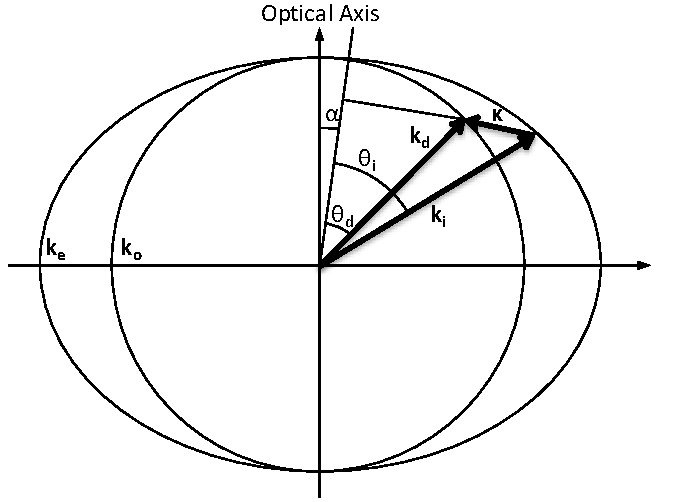
\includegraphics[width=0.7\textwidth]{./Images/3-1-AOTFWavevectorWithRefraction.pdf}
    \caption{The wave vectors generated by the AOTF experiment. The wave vectors are $k_{e}$ and $k_{o}$ for the extraordinary and ordinary axis of the AOTF crystal. The cut angle is hsown as $\alpha$.}
    \label{fig:3.1:ATOFWavevectors}
    \end{center}
\end{figure}

\begin{figure}
    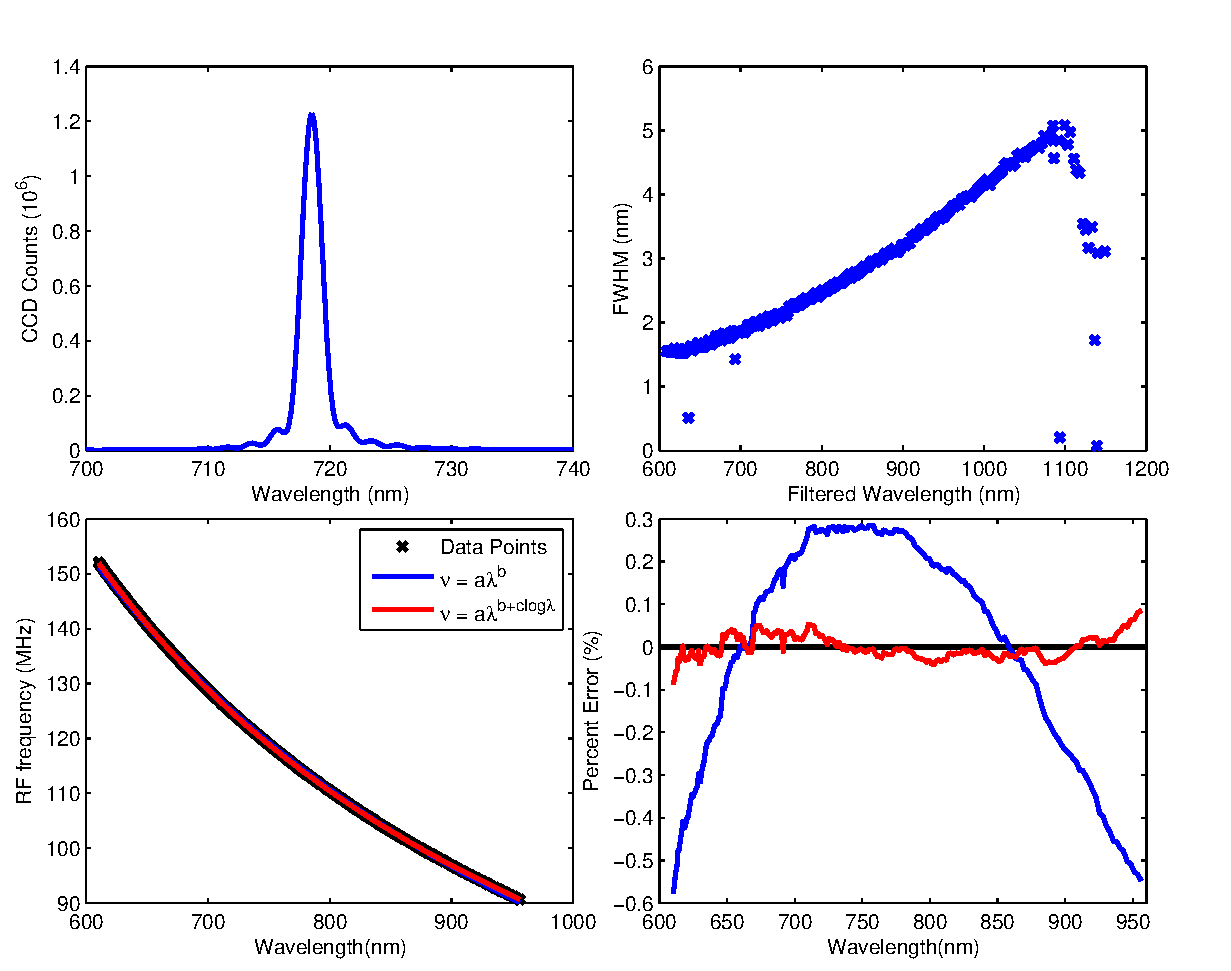
\includegraphics[width=1.0\textwidth]{./Images/3-1-AOTFCharaterization.pdf}
    \caption{Top Left: A standard image taken from the AOTF calibration experiment when the tuning frequency of the AOTF was at 124.96~MHz. Top Right: The FWHM for each of the determined wavelengths for the AOTF. It should be noted that the FWHM at 600~nm is 1.5~and as the wavelengths get longer the FWHM increases to 4.9 at 1080~nm. Bottom Left: The calibration curves for the AOTF RF versus the  diffracted wavelength which contains the data points recorded and two best fit curves. Bottom Right: The percent error with respect to the measured frequency for the two best fit curves in the previous panel.}
    \label{fig:3.1:AOTFCharaterization}
\end{figure}

\begin{figure}
    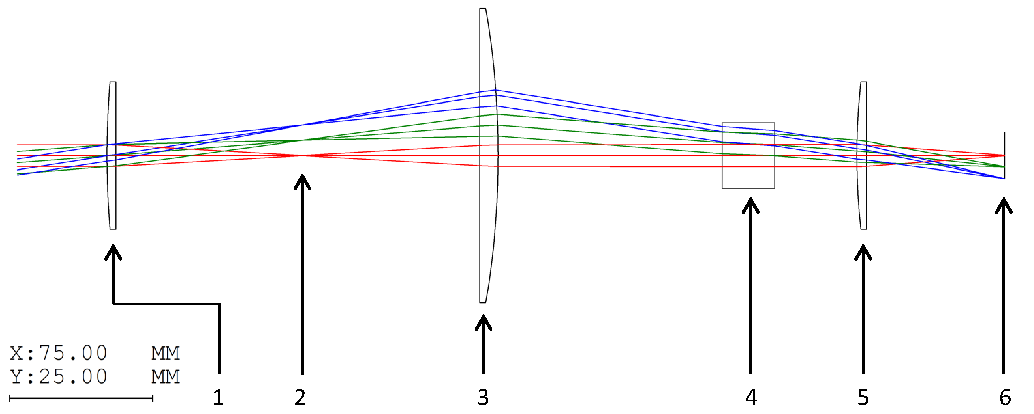
\includegraphics[width=1.0\textwidth]{./Images/3-2-TelescopicRayTracing.pdf}
    \caption{Ray Tracing diagram of the telescopic lens system for ALI simulated by Code V. The elements in the system are the following: (1) 100~mm focal length plano-convex lens. (2) Baffle inserted here to remove unwanted signal. (3) 100~mm focal length plano-convex lens. (4) Linear polarizer orientated to allows vertical polarization through. (5) Brimrose AOTF. (6) Linear polarizer orientated to allows horizontal polarization through. (7) 75.6~mm focal length plano-convex lens. (8) Imaging plane. It should be noted that the x and y scales are not the same in this image.}
    \label{fig:3.2:telescopicRayTracing}
\end{figure}

\begin{figure}
    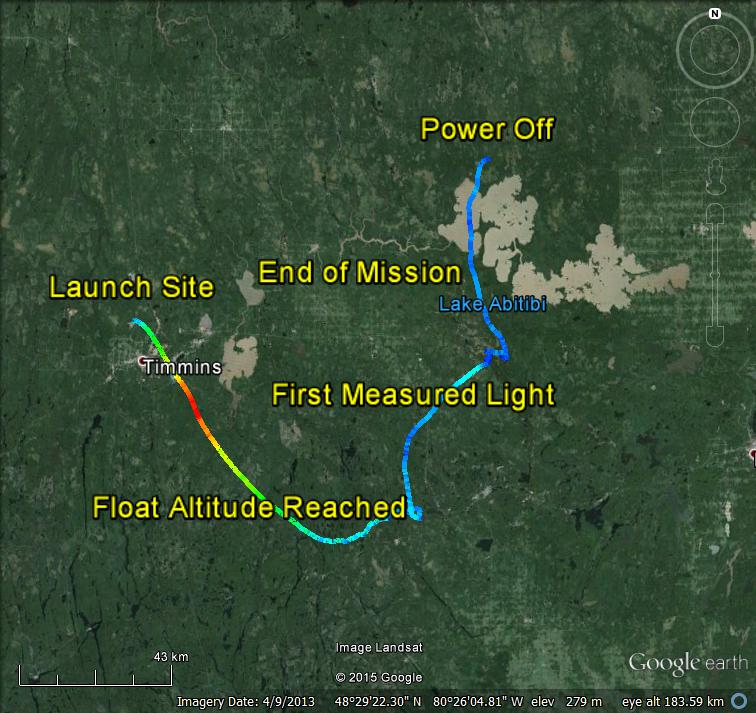
\includegraphics[width=1.0\textwidth]{./Images/5-1-AliGpsDataGoogleMaps.jpg}
    \caption{The GPS data from ALI during the Nimbus 7 mission generated via Google Earth. The colour of the line represents the absolute speed of the gondola during the mission. Important landmarks noted on the image. The end of mission represent the end of the primary aerosol mission. No GPS data was collected from ALI after the power down.}
    \label{fig:5.1:nimbus7FlightPath}
\end{figure}

\begin{figure}
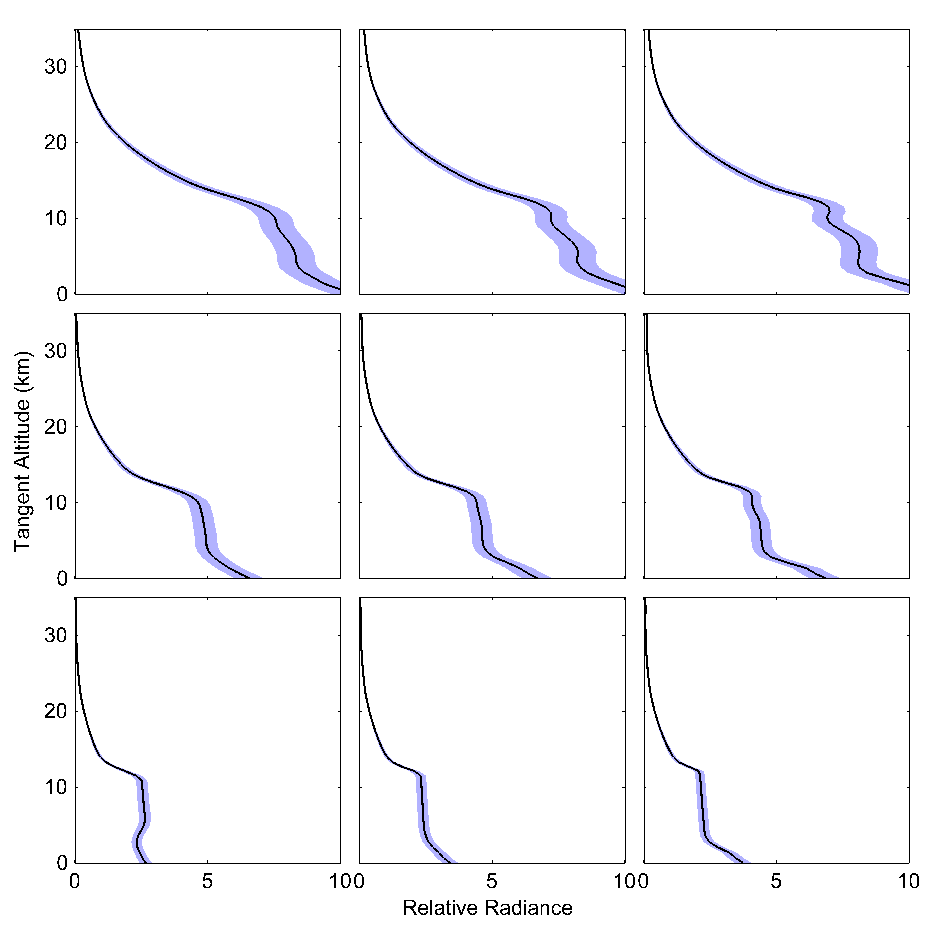
\includegraphics[width=1.0\textwidth]{./Images/AliRadiances.pdf}
    \caption{Level 1 relative radiances as measured form ALI at approximately 14:20 (images number 207, 211,and 215) UTC looking 90\si{\degree} from the sun facing southwards. The top middle, and bottom row are measurements taken at 725~nm, 825~nm, and 925~nm respectively. The center column is viewing the atmosphere directly in front of ALI, While the left column is looking to the left at -2.5\si{\degree} and the right at 2.5\si{\degree}. }
    \label{fig:AliRadiances}
\end{figure}

\begin{figure}
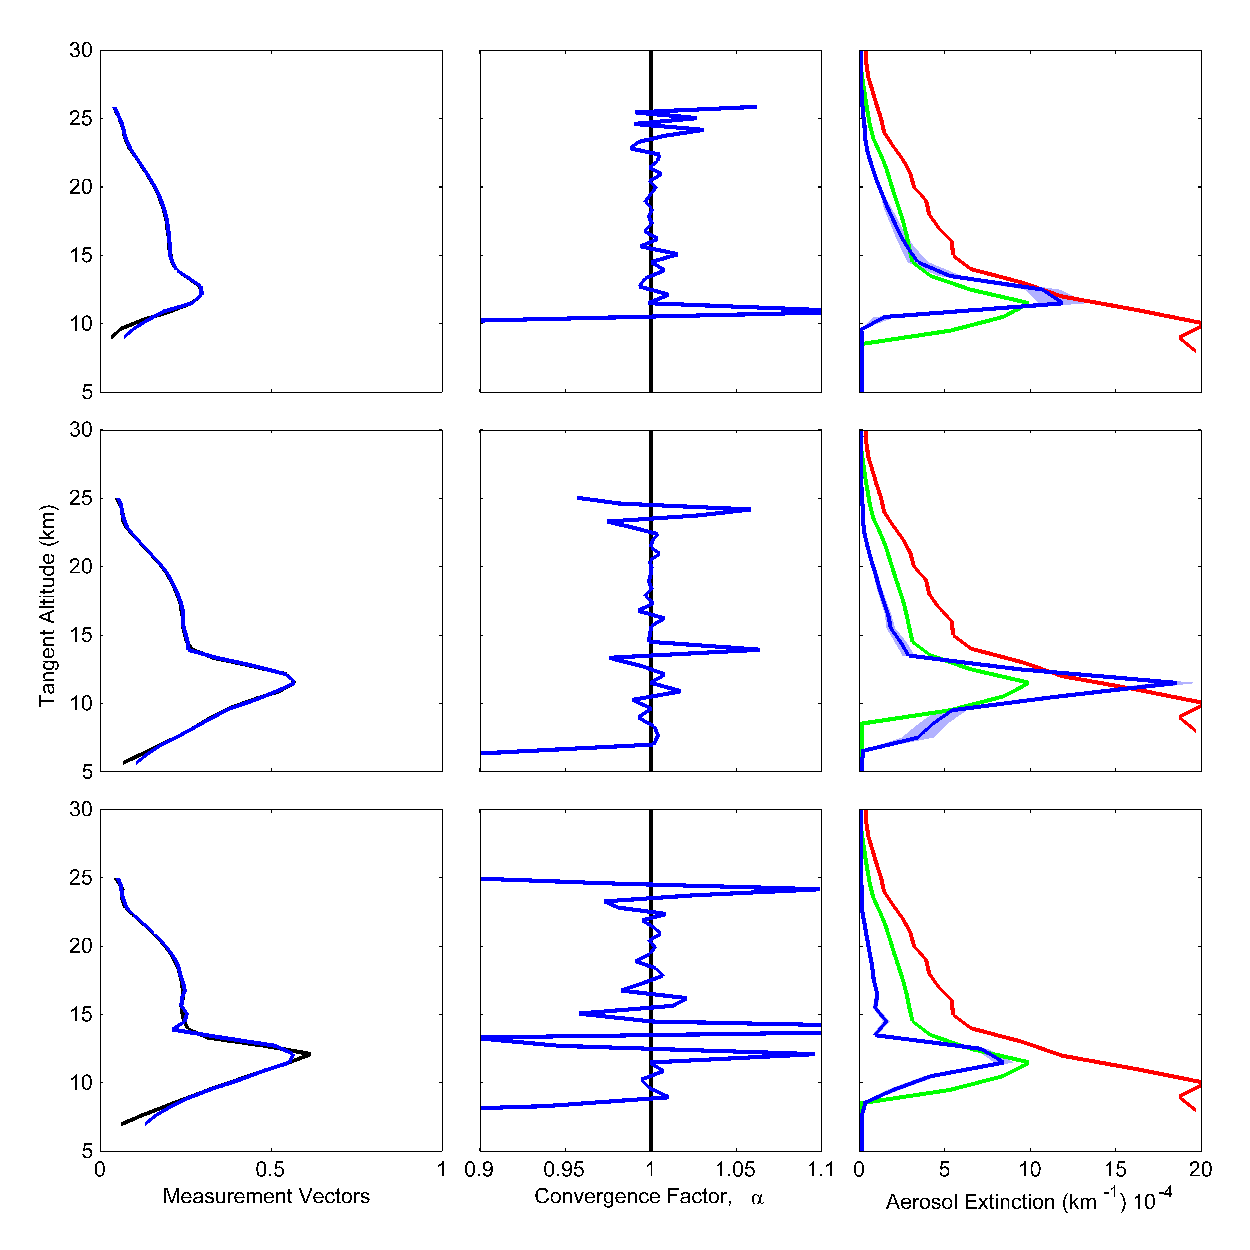
\includegraphics[width=1.0\textwidth]{./Images/AliRetreivals.pdf}
    \caption{An example of three aerosol retrievals from images 207, 211, and 215, with center wavelengths of 725, 825, and 925~nm respectively and vertically displayed in the figure. The left column shows the measurement vector in black with the retrieved foreword model in blue. The center column shows the ratio of the $y$ over $F$ known as $\alpha$ and is the convergence factor between the ALI measurement and the foreword model. The final column is the aerosol extinction in blue with the associated error represented by the light blue shading. The green is aerosol extinction at 750~nm measured by OSIRIS , and red is 750~nm extinction as measure by SOLAMON.}
    \label{fig:AliRetreivals}
\end{figure}

\begin{figure}
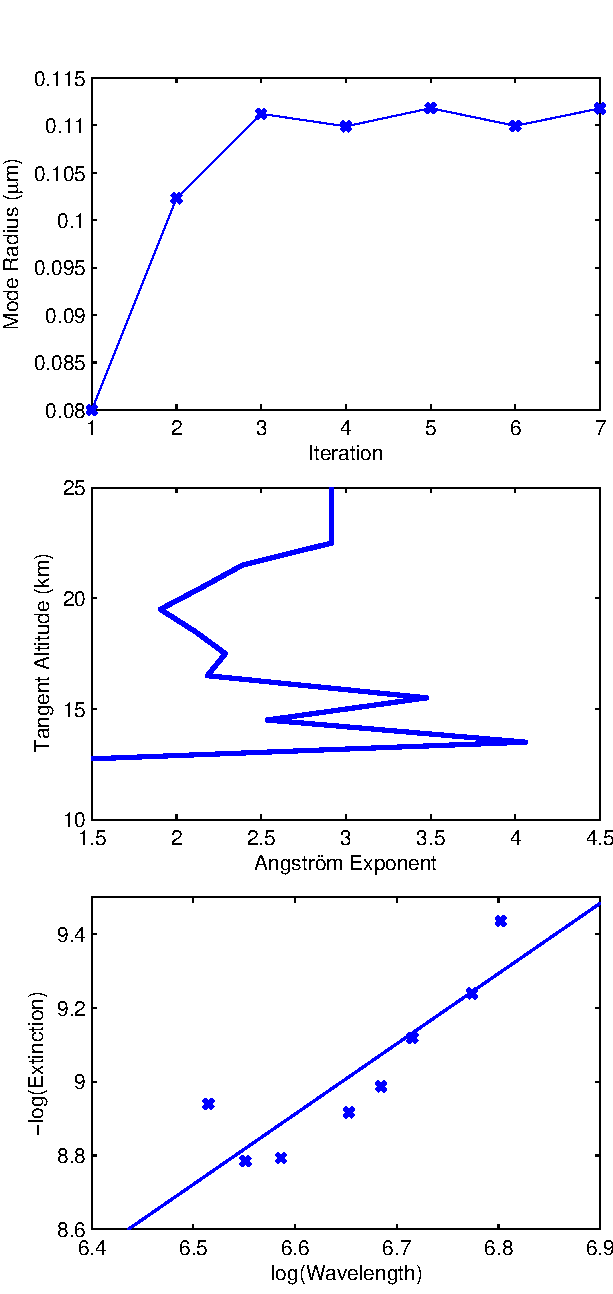
\includegraphics[width=0.5\textwidth]{./Images/ParticelSize.pdf}
    \caption{The top panel shows the convergence of the mode radius through out the iterations in the retrieval. The second panel is the final angstrom exponents determined for images 204-217 during the Timmins 2014 campaign. And the last panel demonstrate a least squares fit to determine the angstrom exponent at 20.5~km shell altitude.}
    \label{fig:ParticleSize}
\end{figure}



\end{document} 